\documentclass[och, master, pract]{SCWorks_fix}

\usepackage[T2A]{fontenc}
\usepackage[utf8]{inputenc}
\usepackage[russian]{babel}

\usepackage{pdfpages}

\usepackage{hyperref}
\usepackage{amsfonts}
\usepackage{commath}
\usepackage{amsthm}
\usepackage{amssymb}
\usepackage{float}
\usepackage{listings}

\theoremstyle{plain}
\newtheorem{thethm}{Теорема}

\theoremstyle{plain}
\newtheorem{lemma}{Лемма}

\theoremstyle{plain}
\newtheorem{note}{Замечание}

\theoremstyle{definition}
\newtheorem{defn}{Определение} 

\newtheorem{exmp}{Пример}

\geometry{verbose,a4paper,tmargin=2cm,bmargin=2cm,lmargin=2.5cm,rmargin=1.5cm}

\hypersetup{
    colorlinks=true, %set true if you want colored links
    linktoc=all,     %set to all if you want both sect. and subsect. linked
    linkcolor=blue,  %choose some color if you want links to stand out
}

\author{Sharov Alex}

\newtheorem{problem}{Проблема}

\begin{document}

%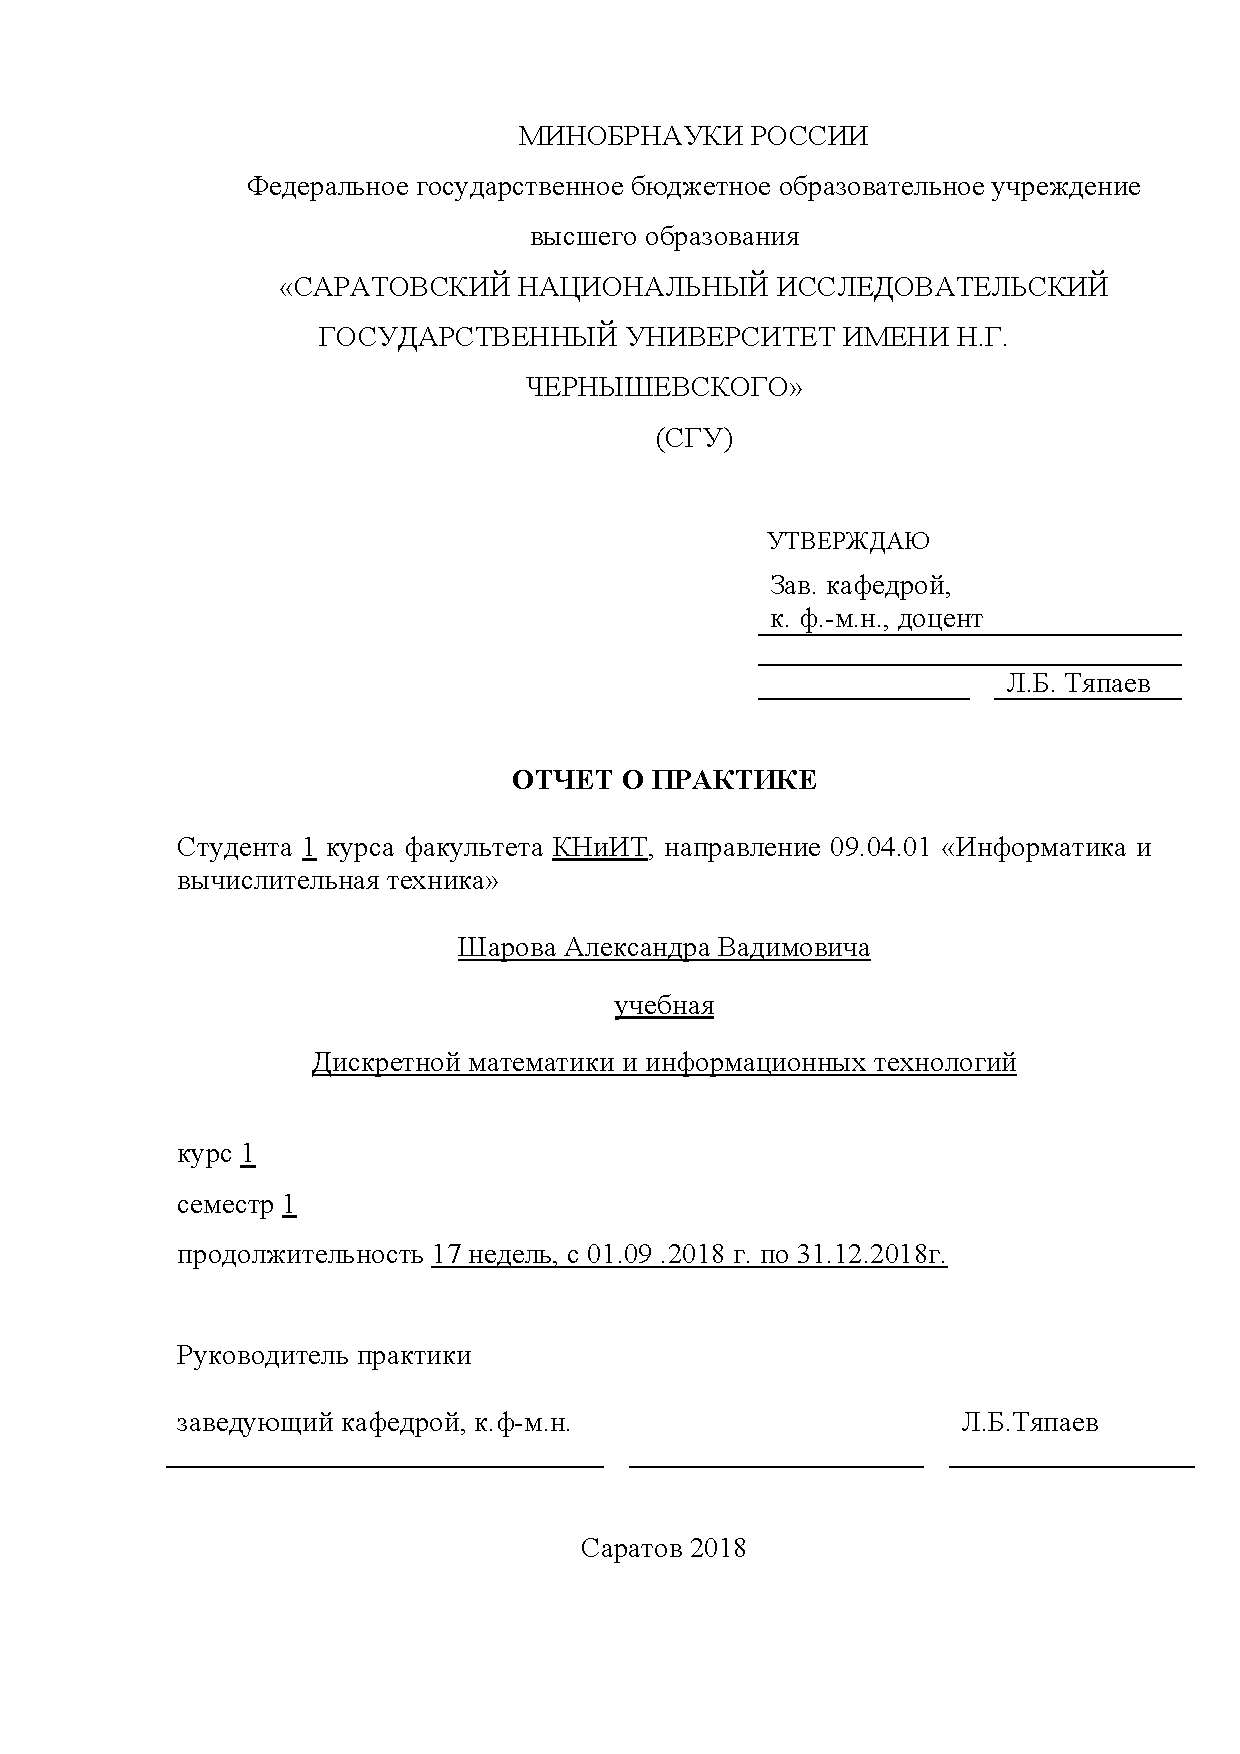
\includepdf[pages={1}]{titul.pdf}
\setcounter{tocdepth}{2}




\chair{дискретной математики и информационных технологий}
%​\title{Математические модели генераторов псевдослучайных чисел}
\course{2}
\group{271}
​\napravlenie{09.04.01 "--- Информатика и вычислительная техника}
\author{Шарова Александра Вадимовича}
​\chtitle{к.ф.-м.н., доцент}
\chname{Л.\,Б.\,Тяпаев}
​\satitle{зав. каф., к.ф.-м.н., доцент}
\saname{Л. Б. Тяпаев}
\term{3}
​\practtype{научно-исследовательская}
\duration{4}
\practStart{07.10.2019}
\practFinish{04.11.2019}
\date{2019}
\maketitle
\tableofcontents

\intro


В настоящий момент криптовалюты повсеместно привлекают к себе высокий интерес, помимо коммерческого вопроса и желания заработать крупный бизнес и обычные люди обратили свое внимание и на технологию, на которой все основано – блокчейн.

Блокчейн – это именно та цифровая платформа, которая даёт концептуальные возможности для безопасного, быстрого и недорогого в обслуживании обращения новой формы денежных средств.\cite{bib:block:1}

Благодаря этому изучение технологии Блокчейн приобретают особую актуальность.

Цель данной научно-исследовательской практики посвящена изучению технологии blockchain и разработке простейшего приложения для работы с данной технологией на языке программирования Golang, который будет выполнять все основные операции.

\section{Технология blockchain}

\begin{defn}
Блокчейн (blockchain) – это распределенная база данных, хранящая данные о совершенных транзакциях (действиях), которые записываются в определенном порядке и формируют неизменную последовательность связанных блоков. Блок – своего рода папка, в которую вложена закодированная информация о контрактах и сделках внутри системы. У этой папки есть свои атрибуты, которые невозможно подделать и которые содержат информацию о предыдущей папке в цепи. У такого атрибута есть специальное название – хеш. Создание блоков получило название майнинг, вознаграждение за успешную работу – специальная криптовалюта - биткоин. \cite{bib:block:4}
\end{defn}

\begin{defn}
Биткоин (bitcoin) – децентрализованная платёжная система, использующая одноимённую единицу для учёта операций и одноимённый протокол передачи данных. Для обеспечения функционирования и защиты системы используются криптографические методы.
\end{defn}

\begin{defn}
Майнинг (mining) – деятельность по созданию новых структур для обеспечения функционирования криптовалютных платформ. За создание очередной структурной единицы обычно предусмотрено вознаграждение за счёт новых (эмитированных) единиц криптовалюты и/или комиссионных сборов. Зачастую майнинг сводится к серии вычислений с перебором параметров для нахождения хеша с заданными свойствами. 
\end{defn}

\subsection{Принцип работы blockchain}

Цифровые записи объединяются в «блоки», которые потом связываются криптографически и хронологически в «цепочку» с помощью сложных математических алгоритмов. Каждый блок связан с предыдущим и содержит в себе набор записей. Новые блоки всегда добавляются строго в конец цепочки. Процесс шифрования, известный как хеширование, выполняется большим количеством разных компьютеров, работающих в одной сети. Если в результате их расчетов все они получают одинаковый результат, то блоку присваивается уникальная цифровая сигнатура (подпись). Как только реестр будет обновлён и образован новый блок, он уже больше не может быть изменён. Таким образом подделать его невозможно. К нему можно только добавлять новые записи. Важно учесть то, что реестр обновляется на всех компьютерах в сети одновременно.

Одна из классических задач криптологии «задача византийских генералов» формулируется следующим образом – «Византийская армия осаждает город. Генералам необходимо выработать единую стратегию действий, которая приведет к победе, даже если среди них будут предатели, намеренно искажающие информацию о численности своих отрядов и времени наступления».

Основная цель задачи выяснить, как согласовать действия участников системы, объединенных одной целью, но лишенных доверия друг к другу.

Если не пользоваться инструментами математики, то очевидным решением кажется создание единого контролирующего и проверяющего органа, который будет гарантировать участникам системы достоверность получаемой информации.
 
Благодаря блокчейн-технологии необходимость в посредниках отпадает. Это достигается благодаря особой форме хранения информации о транзакциях сразу на всех компьютерах системы – в распределенных реестрах или базах данных.

В 2008 году Сатоси Накамото изобрел новый способ достижения социального консенсуса, позволяющий подтверждать истинность всех транзакций без участия третьей стороны. Проще всего продемонстрировать это, вкратце объяснив суть работы блокчейн-технологий на примере переводов в биткоинах.

Каждая транзакция происходит онлайн и представляет собой лишь сообщение о том, что некий пользователь переводит другому пользователю известное количество биткоинов. Как только транзакция проведена, она становится видна майнерам.

Ни одна из транзакций не будет считаться завершенной, пока ее не включат в так называемый блок – именно этим и занимаются майнеры. Каждый блок содержит информацию о тысячах обрабатываемых транзакций. Чтобы он считался сформированным, майнер должен вычислить хеш-функцию – цифробуквенную строку, в которую преобразован входящий массив данных.

Хеш-функция содержит информацию о предыдущем блоке, а значит – обо всех транзакциях, совершенных с момента возникновения биткоина как валюты. Если изменить хотя бы бит информации в предыдущей цепочке, до неузнаваемости изменится и хеш-функция. Получается, что распределенная база данных в блокчейне – это цепочка из блоков, каждый из которых ссылается на предыдущий.

Сохранение истории операций с биткоинами гарантирует, что пользователь не переведет кому-то сумму, которой у него нет. Блокчейн-технология позволяет избежать и двойного расходования – ситуации, когда человек дважды пытается потратить одну и ту же сумму. Залогом этого служит большое количество пользователей и майнеров.

Разберем подробнее понятие хеш-функции, на котором строится безопасность блокчейна.

\subsection{Хеширование}
\begin{defn}
Хеширование – это процесс преобразования массива входных данных произвольной длины в (выходную) битовую строку фиксированной длины. Например, хеш-функция может принимать строку с любым количеством знаков (одна буква или целое литературное произведение), а на выходе получать строку со строго определенным числом символов (дайджест).
\end{defn}

Хеш используется для того, чтобы быстрее отличать одни данные от других без необходимости сравнивать каждый бит этих данных. Достаточно обработать эти данные один раз (вычислить их хеши) и можно сравнивать только их, а это гораздо быстрее. Идея заключается в том, что, если хеши различаются, значит, это совершенно точно разные данные. Если хеши одинаковы, значит, с вероятностью в 99.9 процентов это одинаковые данные. Хотя всегда существует маленький шанс, что данные всё-таки разные, несмотря на одинаковые хеши.

Требования, которые выдвигаются для хеширующего алгоритма (хеш-функции):

1) Одни и те же данные должны давать всегда один и тот же хеш. Это обязательное условие.

2) Разные данные должны давать разный хеш. 

\noindentХорошая хеш-функция ведёт себя следующим образом:

1) Весь доступный диапазон хешей используется по максимуму. То есть, если на хеш отведено 32 байта, то разные данные дают максимально разнообразный хеш, который может являться совершенно любой комбинацией битов. 

2) Любое, даже самое незначительное, изменение входных данных должно давать другой хеш. Не должно быть такого, что небольшие изменения дают тот же самый хеш. Тот же самый хеш должен возникать в результате какого-то совершенно другого набора данных, чтобы вероятность случайного присутствия двух таких данных (дающих одинаковый хеш) была минимальной.
 	
Для чего нужен хеш. Предположим, есть массив из миллиона разных строк. В каждой строке миллион символов (то есть, всего 1 терабайт = 1000 гигабайт данных). Вам приходит такое указание: добавьте строку, содержащую какую-либо информацию в ваш массив, но только в том случае, если такой строки там ещё нет.

В итоге, задача превращается в посимвольное сравнение миллиона символов в миллионах строк. Очевидно, что данная работа потребует огромное количество ресурсов и времени.

Но если перед записью имеются вычисленные заранее хеши эти строк, то задача превращается в сравнение 32 символов вместо миллиона символов (32 мегабайта данных на весь массив). Если будет обнаружено, что в списке есть точно такой же хеш, то для полной надёжности, можно сравнить посимвольно лишь эту строку. 

Хеш-функции в блокчейнах гарантируют «необратимость» всей цепочки транзакций. Дело в том, что каждый новый блок транзакций ссылается на хеш предыдущего блока в реестре. Хеш самого блока зависит от всех транзакций в блоке, но вместо того, чтобы последовательно передавать транзакции хеш-функции, они собираются в одно хеш-значение при помощи двоичного дерева с хешами (дерево Меркла). Таким образом, хеш используются как замена указателям в обычных структурах данных: связанных списках и двоичных деревьях. За счет использования хешей общее состояние блокчейна – все когда-либо выполненные транзакции и их последовательность – можно выразить одним-единственным числом: хешем самого нового блока. Поэтому свойство неизменности хеша одного блока гарантирует неизменность всего блокчейна.\cite{bib:block:2}

Хеш-деревья имеют много применений помимо блокчейнов. Они используются в файловых системах для проверки целостности файлов, распределенных базах данных для быстрой синхронизации копий и в управлении ключами для надежного журналирования выдачи сертификатов. Git использует обобщение хеш-деревьев – направленные ациклические графы на основе хешей. В блокчейне использование хеш-деревьев продиктовано соображениями производительности, так как они делают возможным существование «легких клиентов», которые обрабатывают лишь малую часть транзакций из блокчейна.

\subsection{Цифровая подпись}
\begin{defn}
Цифровая подпись – это последовательность байтов, формируемая путем преобразования подписываемой информации по криптографическому алгоритму и предназначенная для проверки авторства электронного документа.\cite{bib:block:3}
\end{defn}

Цифровые подписи, так же, как и настоящие подписи, – это один из способов доказать, что кто-то является тем, за кого он себя выдает. С учетом того, что в этой ситуации используется криптография и математика, это значительно безопаснее, чем обычные рукописные подписи, которые можно легко подделать.

В асимметричных системах шифрования пользователи генерируют по определенному алгоритму так называемые пары ключей, каждая из которых является открытым ключом (public key) и закрытым ключом (private key).

Открытый и закрытый ключи связаны друг с другом при помощи некоторых математических отношений. Открытый ключ предназначен для распространения публично. Он служит в качестве адреса для приема сообщений от других пользователей, таких как IP-адрес или домашний адрес.

Закрытый ключ хранят в секрете. Он используется в качестве цифровой подписи для сообщений, отправленных другим пользователям. Подпись включается в сообщение, таким образом, получатель может идентифицировать отправителя с помощью его открытого ключа.

Цифровые подписи в блокчейне базируются на криптографии с открытым ключом. В ней используются два ключа. Первый – закрытый ключ – нужен для формирования цифровых подписей. Второй – открытый ключ – используется для проверки электронной подписи. Открытый ключ реально вычислить на основе закрытого ключа, а вот обратное преобразование требует невозможного на практике объема вычислений. 

Поскольку в блокчейне нет центрального узла, который может авторизовать произвольные транзакции, безопасность системы становится децентрализованной, а вероятность успешного вмешательства в работу блокчейна снижается практически до нуля. Таким образом, блокчейн использует цифровые подписи для аутентификации и обеспечения целостности транзакций (и иногда блоков). В случае криптовалюты процесс аутентификации означает, что потратить средства может только тот человек, которому они были посланы другой, более ранней, транзакцией. Особенность блокчейна состоит в том, что информация об аутентификации «вшита» в каждую транзакцию, а не отделена от бизнес-логики, поэтому блокчейн считается более защищенным. В обычной системе можно взломать или административно обойти механизм аутентификации и провести манипуляции с бэкэндом, а в блокчейне сделать этого не получится по определению.

\section{Достоинства технологии блокчейн}

Именно в отсутствии посредников и заключается главное преимущество блокчейна перед обычными банковскими транзакциями\cite{bib:block:5}. Известно, что сейчас все операции с документами, деньгами или иными данными обязательно проходят через посредников. Государственные органы, банки или нотариусы постоянно следят за подлинностью проделанных операций. Здесь же не имеется центрального органа, поэтому транзакции проверяют все участники системы. Это значительно упрощает процедуру и избавляет от посредников.

Программный код сети доступен любому желающему обратиться к нему, однако личность пользователя и иная персональная информация не раскрывается. Создателям блоков видны только необходимые данные по конкретной операции. 

Блокчейн децентрализован, нет какого-то одного общего командного центра, взломав который получится уничтожить все данные о сделке и ее участниках или подменить их.

Например, если проводилась транзакция, в которой участвовали 100 человек, то эта блокчейн-цепочка останется рабочей и доступной для просмотра даже в том случае, если 99 компьютеров других участников будут испорчены. Ведь, по сути, каждое звено блокчейн-цепи – это своеобразный полный бекап данных всех транзакций всех остальных участников на это звено.
 	Взлом одного из таких компьютеров никак не скажется на сохранности данных на остальных (как и на их изменении).

\subsection{Основные принципы обеспечения безопасности}

Применение шифрования гарантирует, что пользователи могут изменять только те части цепочки блоков, которыми они «владеют» в том смысле, что у них есть закрытые ключи, без которых запись в файл невозможна. Кроме того, шифрование гарантирует синхронизацию копий распределенной цепочки блоков у всех пользователей. В технологию блокчейн изначально заложена безопасность на уровне базы данных. Концепцию цепочек блоков предложил в 2008 г. Сатоши Накамото (Satoshi Nakamoto). Впервые реализована она была в 2009 г. как компонент цифровой валюты – биткоина, где блокчейн играет роль главного общего реестра для всех операций с биткоинами. Благодаря технологии блокчейна биткоин стал первой цифровой валютой, которая решает проблему двойных расходов (в отличие от физических монет или жетонов, электронные файлы могут дублироваться и тратиться дважды) без использования какого-либо авторитетного органа или центрального сервера.

Безопасность в технологии блокчейн обеспечивается через децентрализованный сервер, проставляющий метки времени, и одноранговые сетевые соединения. В результате формируется база данных, которая управляется автономно, без единого центра. Это делает цепочки блоков очень удобными для регистрации событий (например, внесения медицинских записей) и операций с данными, управления идентификацией и подтверждения подлинности источника.

Блокчейн-технология имеет встроенную устойчивость к ошибкам. Это служит хорошим предзнаменованием для блокчейн-технологии, которая продолжает развиваться. Как бы революционно это ни звучало, блокчейн действительно представляет собой механизм, обеспечивающий высшую степень учета и идентификации. Больше не будет пропущенных транзакций, ошибок человека или машины, или даже изменений, сделанных без согласия вовлеченных сторон. А наиболее важно то, что блокчейн помогает гарантировать законность транзакции путем записи её не только в главном реестре, а в распределённой системе реестров, связанных через защищенный механизм проверки.

\subsection{Сферы применение технологии в реальной жизни}
Неизменные и верифицированные данные, прозрачность правоотношений, быстрота и удобство сервиса – все эти причины стали поводом для того, чтобы крупный бизнес обратил внимание на эту перспективную технологию. Как прогнозирует Json & Partners Consulting, первые кандидаты на внедрение блокчейна – финансовая сфера, телеком, транспорт, промышленность и агропромышленный комплекс.

Кстати, банки понимают все перспективы блокчейн и активно начинают использовать его. Например, в России создание блокчейн-платформ тестируют Сбербанк, банки Тинькофф, Открытие, Альфа и платежная система Qiwi. Технические решения на основе блокчейн разрабатывает ЦБ. Есть первые тестовые транзакции.

Несмотря на то, что интерес к Блокчейн-технологии в большей степени связан скорее с областью финансов, сферы применения технологии распределенных реестров не ограничиваются только ей. Наряду с банками, игроки других, не связанных с финансовой отраслью рынков, также обратили внимание на технологию и ищут способы извлечения пользы из возможностей, которые она предоставляет.


\conclusion
В дальнейшей научной работе планируется интеграция средств $p$-адического анализа в простейшие виды блокчейнов в виде алгоритма предназначенного для подписания блоков в цепочках.


\bibliographystyle{biblio/ugost}
\bibliography{biblio/biblio}


\appendix
\section{Исходный код реализации}

\lstinputlisting[language=c, numbers=left, showstringspaces=false, breaklines=true, basicstyle=\scriptsize]{code/blockchain.go}


\end{document}